% Create a Table of Contents in Beamer
\documentclass[10pt,t]{beamer}
% Theme choice:
\usetheme{Singapore}
\useoutertheme{sidebar}
\usecolortheme{seahorse}
\setbeamercolor{titlelike}{bg=white}
\setbeamercolor{frametitle}{bg=white}
%\setbeamertemplate{frametitle}[default][left]
\setbeamertemplate{navigation symbols}{}

\usepackage{graphicx}
\usepackage{amsmath}
\usepackage{amsfonts}
\usepackage{amssymb}
\usepackage{amsthm}
\usepackage{ulem}
\usepackage{listings}
\usepackage{xcolor}
\usepackage{wrapfig}
\usepackage{subfig}
\usepackage{setspace}
\usepackage{enumerate}
\usepackage{verbatim}
\usepackage{tikz}

% new amber color
\definecolor{amber}{rgb}{1.0, 0.75, 0.0}

% Title page details: 
\title{Bonus Lecture: Spatial Statistics and Under-5 Mortality Estimation} 
\author{Taylor Okonek}
\date{\today}


\begin{document}
	% Title page frame
\begin{frame}
	\titlepage 
\end{frame}


% Outline frame
\begin{frame}{Outline}
	\tableofcontents
\end{frame}

\AtBeginSection[ ]
{
	\begin{frame}{Outline}
		\tableofcontents[currentsection]
	\end{frame}
}


\section{Under-5 Mortality Estimation}

\subsection{Why does this matter?}

\begin{frame}{Millennium Development Goals}
The Millennium Development Goals (MDGs) for the year 2015 were established in 2000 by the United Nations, and aimed to achieve the following:
\vspace{0.3cm}

\begin{enumerate}
	\item To eradicate extreme poverty and hunger
	\item To achieve universal primary education
	\item To promote gender equality and empower women
	\item To reduce child mortality
	\item To improve maternal health
	\item To combat HIV/AIDS, malaria, and other diseases
	\item To ensure environmental sustainability
	\item To develop a global partnership for development
\end{enumerate}
\end{frame}

\begin{frame}{Millennium Development Goals}
The Millennium Development Goals (MDGs) for the year 2015 were established in 2000 by the United Nations, and aimed to achieve the following:
\vspace{0.3cm}

\begin{enumerate}
	\item To eradicate extreme poverty and hunger
	\item To achieve universal primary education
	\item To promote gender equality and empower women
	\item \textcolor{orange}{To reduce child mortality}
	\item To improve maternal health
	\item To combat HIV/AIDS, malaria, and other diseases
	\item To ensure environmental sustainability
	\item To develop a global partnership for development
\end{enumerate} \pause

\end{frame}

\begin{frame}{Millenium Development Goals}
Within each of the eight MDGs, there were specific targets that quantified how each goal would be considered ``met"\dots \pause

\vspace{0.3cm}

\textcolor{blue}{Target 4A: Reduce by two-thirds, between 1990 and 2015, the under-five mortality rate} \pause

\vspace{0.3cm}

In 2004, the United Nations Inter-agency Group for Child Mortality Estimation (\href{https://childmortality.org/}{\textcolor{cyan}{UN IGME}}) was formed to:

\vspace{0.3cm}

\begin{itemize}
	\item assess whether Target 4A (among other within MDG 4) was on track to be met
	\item improve methods for child mortality estimation
	\item share data on child mortality estimates
\end{itemize}

\end{frame}

\begin{frame}{Target 4A}
How did countries do with Target 4A?

\vspace{0.3cm}

Out of 1000 live-births from 1990 to 2015:

\vspace{0.3cm}

\begin{itemize}
	\item Sweden: 6.97 to 2.86 deaths (59\% reduction)
	\item USA: 11.22 to 6.79 deaths (39\% reduction)
	\item Bangladesh: 146.15 to 38.07 deaths (74\% reduction)
	\item Nigeria: 210.05 to 126.45 deaths (40\% reduction)
\end{itemize}



\end{frame}

\begin{frame}{UN IGME Visualizations}
\centering 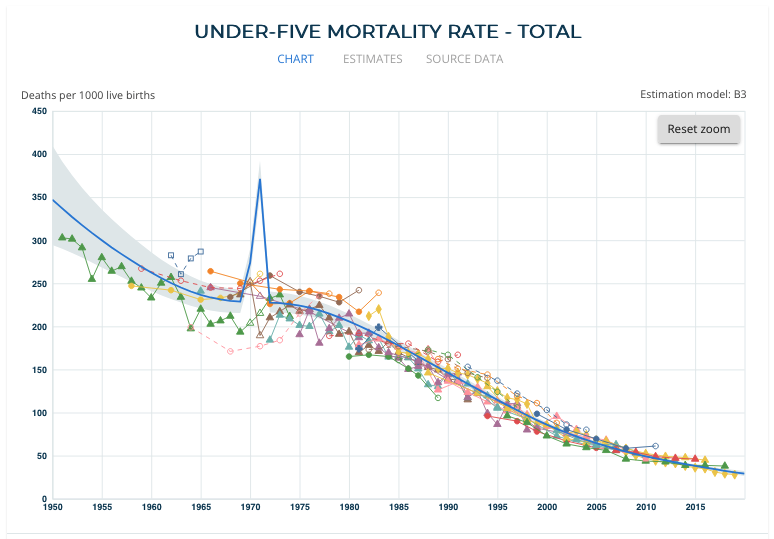
\includegraphics[scale=0.3]{bangladesh_igme.png}
\end{frame}

\begin{frame}{Target 4A}
How did countries do with Target 4A?

\vspace{0.3cm}

Out of 1000 live-births from 1990 to 2015:

\vspace{0.3cm}

\begin{itemize}
	\item Sweden: 6.97 to 2.86 deaths (59\% reduction)
	\item USA: 11.22 to 6.79 deaths (39\% reduction)
	\item Bangladesh: 146.15 to 38.07 deaths (74\% reduction)
	\item Nigeria: 210.05 to 126.45 deaths (40\% reduction)
\end{itemize}

\vspace{0.3cm} 

Progress towards Target 4A varied quite a bit by country, a lot of which had to with valid criticisms of the MDGs as a whole and issues related to financial support received by individual countries from world government organizations.

\end{frame}

\begin{frame}{Sustainable Development Goals}
The MDGs were goals set for 2015, so what about post-2015? 
\vspace{0.3cm}

The UN established the Sustainable Development Goals (SDGs) in 2015 for the target year 2030, to address 17 different goals. These goals are broad and related to one another in some ways, but similar to the MDGs, include specific targets that are meant to be achieved by 2030.

\vspace{0.3cm}

One of the overarching themes of the SDGs (as stated by the UN Secretary General in 2015) is the need for a \textit{Data Revolution for Sustainable Development}. The aim is to improve ``coverage, quality, availability and timeliness of data used to measure and monitor progress toward the SDGs."

\end{frame}

\begin{frame}{Sustainable Development Goals}
SDG 3: Good health and well-being

\vspace{0.3cm}

\begin{itemize}
	\item One of the targets for SDG 3: End all \textcolor{blue}{preventable} deaths of newborns and children under 5 years of age, reduce neonatal mortality to 12 deaths per 1000 live births or lower, and reduce under-5 mortality to 25 deaths per 1000 live births or lower 
\end{itemize}

\vspace{0.3cm}

\pause As of 2021, 195 countries have already met this target. However, UN IGME estimates that if current trends continue, 54 countries will not meet the under-5 mortality target by 2030, and 61 countries will not meet the under-5 mortality target by 2030.

\vspace{0.3cm}

\pause Where can we come in (as biostatisticans) to help countries meet this target, and lower child mortality rates in general?
\end{frame}

\subsection{Why do we need fancy statistical methods?}

\begin{frame}{Child mortality data}
Child mortality data comes in different formats. Just as we've talked in BIOST 311 about different types of study designs, there are also different methods of collecting mortality data!

\vspace{0.3cm}

\begin{itemize}
	\item \textcolor{blue}{Vital registration}: births and deaths are recorded for everyone in a population, including dates for each of these events
	\item \textcolor{blue}{Full birth history}: births and deaths are recorded for a subset of the population, including dates for each of these events
	\item \textcolor{blue}{Summary birth history}: births and deaths are recorded for a subset of the population, but dates are not collected
\end{itemize}

\vspace{0.3cm}

\pause Vital registration data is most complete data on births and deaths that we can have, but \textit{many} low and middle income countries do not have accurate vital registration data. For these countries, we need to estimate mortality rates from full and summary birth histories.
% vital registration, full birth history, summary birth history (census)
% UN IGME reports that almost 2/3 of low and middle income countries have no reliable mortality data in the past three years (this is 2018-2021) (aka no vital registration)
\end{frame}

\begin{frame}{Full and summary birth history data}
Both full and summary birth history data are typically collected via nationally representative surveys, and summary birth history data is often collected in a census as well.

\vspace{0.3cm}

\textcolor{blue}{Summary birth history data}: Mothers are asked how many children they have ever had, and how many of those children have died

\vspace{0.3cm} \pause

\begin{table}[]
	\begin{tabular}{l|l|l|l}
		\multicolumn{1}{c|}{Mother ID} & \multicolumn{1}{c|}{Mother's Age} & \multicolumn{1}{c|}{No. Children} & \multicolumn{1}{c}{No. Died} \\ \hline
		1                              & 16                                & 1                                 & 0                            \\
		2                              & 22                                & 3                                 & 1                            \\
		3                              & 34                                & 4                                 & 2                            \\
		4                              & 18                                & 2                                 & 0                            \\
		5                              & 25                                & 5                                 & 0                           
	\end{tabular}
\end{table}

\pause Summary birth history data is the most \textit{common} source of child mortality information in low and middle income countries, as it is the ``cheapest" to collect.

\end{frame}

\begin{frame}{Full and summary birth history data}
Both full and summary birth history data are typically collected via nationally representative surveys, and summary birth history data is often collected in a census as well.

\vspace{0.3cm}

\textcolor{blue}{Full birth history data}: Mothers are asked how many children they have ever had, as well as their dates of birth and (possibly) death

\vspace{0.3cm} \pause

\begin{table}[]
	\begin{tabular}{l|l|l|l}
		\multicolumn{1}{c|}{Mother ID} & \multicolumn{1}{c|}{Child ID} & \multicolumn{1}{c|}{DOB} & \multicolumn{1}{c}{DOD} \\ \hline
		1                              & 1                             & Jan 2001                 & NA                      \\
		1                              & 2                             & Mar 2003                 & Apr 2003                \\
		2                              & 1                             & Oct 2002                 & NA                      \\
		3                              & 1                             & Feb 2004                 & Sep 2006                \\
		3                              & 2                             & Feb 2005                 & NA                     
	\end{tabular}
\end{table}

\pause Full birth history data is often the most \textit{reliable} source of child mortality information in low and middle income countries, and is what we will focus on in this lecture!

\end{frame}


\begin{frame}{The Demographic and Health Surveys (DHS) Program}
One of the leading sources of full birth history data for low and middle income countries are the Demographic and Health Surveys (\href{https://dhsprogram.com/}{\textcolor{cyan}{DHS}}). They are designed to provide nationally representative (unbiased) estimates for a variety of demographic indicators. 

\vspace{0.3cm}

As with most surveys, the DHS cannot collect information from every individual in a country. The majority of their surveys to ensure that users of their data are able to make \textit{precise}, unbiased estimates and precictions at the \textcolor{orange}{Administrative 1} level.

\vspace{0.3cm}

\textcolor{orange}{Administrative 1 level}: The largest subnational administrative unit of a country. In the U.S., these are states (and the Administrative 2 level are counties).

\vspace{0.3cm}

\textcolor{blue}{Question:} What do we mean by ensuring precise, unbiased estimates at the Administrative 1 level?

\end{frame}

\begin{frame}{The Demographic and Health Surveys (DHS) Program}
\textcolor{blue}{Question:} What do we mean by ensuring precise, unbiased estimates at the Administrative 1 level?

\vspace{0.3cm}

To get \textbf{unbiased} estimates, we need to assign a weight to each individual in our dataset. The weight for each individual ends up being 1 divided by the probability that they were included in the survey. If we have a simple random sample of individuals, everyone gets an equal weight (this is the simplest case).

\vspace{0.3cm}

To get \textbf{precise} estimates at the Administrative 1 level, we need to have a \textit{large enough} sample size in each Administrative 1 level.

\end{frame}

\begin{frame}{Data sparsity}
Most surveys, including the DHS, are designed to get precise, unbiased estimates at the Administrative 1 level. 

\vspace{0.3cm}

Obtaining \textit{subnational} estimates of quantities like child mortality, disease prevalence, etc. are important for making informed, targeted public health interventions in scenarios where we have limited resources (or decentralized public health infrastructure!)

\vspace{0.3cm}

\textit{However}, public health interventions often take place at the Administrative 2 level. An example of this would be the First Steps program we looked at in Chapter 1, implemented in King County (not the whole state of Washington). In general, estimates at smaller levels of aggregation will be most useful for targeted interventions. 

\vspace{0.3cm}

\pause If we have vital registration data, obtaining reliable estimates at the Administrative 2 level is very straightforward. When we only have access to survey data that is designed to obtain relibale estimates at the Adminstrative 1 level, this gets very complicated very quickly\dots
\end{frame}

\begin{frame}{Data sparsity}

\small To illustrate the issue, suppose we are interested in estimating HIV prevalence at the Administrative 2 level. We collect information on HIV status from a representative sample of individuals. Our survey is designed to get precise estimates at the Administrative 1 level, so our sample size in each Administrative 1 region is large. Each box below represents an Administrative 1 region, and each point represents 1000 people.

\centering
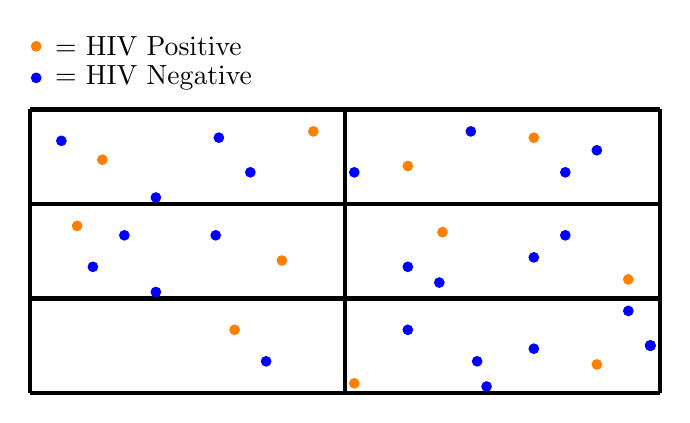
\begin{tikzpicture}[scale=0.4]

\draw[blue,fill=blue] (0.2,12) circle (1ex);
\draw[orange,fill=orange] (0.2,13) circle (1ex);
\node[right] at (0.2,12) {$\text{ = HIV Negative}$};
\node[right] at (0.2,13) {$\text{ = HIV Positive}$};


% Connecting lines LHS
\draw [black, ultra thick] (0,5) -- (20,5);
\draw [black, ultra thick] (0,8) -- (20,8);
\draw [black, ultra thick] (0,11) -- (20,11);
\draw [black, ultra thick] (0,2) -- (20,2);
\draw [black, ultra thick] (0,2) -- (0,11);
\draw [black, ultra thick] (20,2) -- (20,11);
\draw [black, ultra thick] (10,2) -- (10,11);
%\draw [black, ultra thick] (5,2) -- (5,11);
%\draw [black, ultra thick] (15,2) -- (15,11);
% points
\draw[blue,fill=blue] (2,6) circle (1ex);
\draw[blue,fill=blue] (3,7) circle (1ex);
\draw[blue,fill=blue] (4,5.2) circle (1ex);
\draw[blue,fill=blue] (5.9,7) circle (1ex);
\draw[blue,fill=blue] (7,9) circle (1ex);
\draw[blue,fill=blue] (6,10.1) circle (1ex);
\draw[blue,fill=blue] (7.5,3) circle (1ex);
\draw[blue,fill=blue] (1,10) circle (1ex);
\draw[blue,fill=blue] (10.3,9) circle (1ex);
\draw[blue,fill=blue] (12,6) circle (1ex);
\draw[blue,fill=blue] (12,4) circle (1ex);
\draw[blue,fill=blue] (14,10.3) circle (1ex);
\draw[blue,fill=blue] (13,5.5) circle (1ex);
\draw[blue,fill=blue] (14.2,3) circle (1ex);
\draw[blue,fill=blue] (14.5,2.2) circle (1ex);
\draw[blue,fill=blue] (16,3.4) circle (1ex);
\draw[blue,fill=blue] (17,9) circle (1ex);
\draw[blue,fill=blue] (18,9.7) circle (1ex);
\draw[blue,fill=blue] (19,4.6) circle (1ex);
\draw[blue,fill=blue] (19.7,3.5) circle (1ex);
\draw[blue,fill=blue] (19.7,3.5) circle (1ex);
\draw[blue,fill=blue] (19.7,3.5) circle (1ex);
\draw[blue,fill=blue] (19.7,3.5) circle (1ex);
\draw[blue,fill=blue] (17,7) circle (1ex);
\draw[blue,fill=blue] (16,6.3) circle (1ex);
\draw[blue,fill=blue] (4, 8.2) circle (1ex);

\draw[orange,fill=orange] (1.5,7.3) circle (1ex);
\draw[orange,fill=orange] (8,6.2) circle (1ex);
\draw[orange,fill=orange] (2.3,9.4) circle (1ex);
\draw[orange,fill=orange] (9,10.3) circle (1ex);
\draw[orange,fill=orange] (12,9.2) circle (1ex);
\draw[orange,fill=orange] (16,10.1) circle (1ex);
\draw[orange,fill=orange] (13.1,7.1) circle (1ex);
\draw[orange,fill=orange] (19,5.6) circle (1ex);
\draw[orange,fill=orange] (6.5,4) circle (1ex);
\draw[orange,fill=orange] (10.3,2.3) circle (1ex);
\draw[orange,fill=orange] (18,2.9) circle (1ex);

\end{tikzpicture}
\end{frame}

\begin{frame}{Data sparsity}

\small We had a reasonable number of observations in each Administrative 1 region on the previous slide, but if we now split our ``map" into Administrative 2 regions, we can see that one of our Administrative 2 regions has no data! How do we make reasonable, precise estimates for Administrative 2 regions with little to no data? \textcolor{blue}{This is where statistics comes in!}

\centering
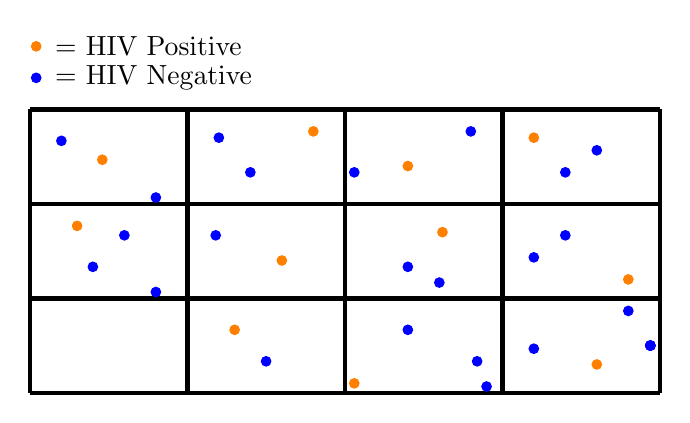
\begin{tikzpicture}[scale=0.4]

\draw[blue,fill=blue] (0.2,12) circle (1ex);
\draw[orange,fill=orange] (0.2,13) circle (1ex);
\node[right] at (0.2,12) {$\text{ = HIV Negative}$};
\node[right] at (0.2,13) {$\text{ = HIV Positive}$};


% Connecting lines LHS
\draw [black, ultra thick] (0,5) -- (20,5);
\draw [black, ultra thick] (0,8) -- (20,8);
\draw [black, ultra thick] (0,11) -- (20,11);
\draw [black, ultra thick] (0,2) -- (20,2);
\draw [black, ultra thick] (0,2) -- (0,11);
\draw [black, ultra thick] (20,2) -- (20,11);
\draw [black, ultra thick] (10,2) -- (10,11);
\draw [black, ultra thick] (5,2) -- (5,11);
\draw [black, ultra thick] (15,2) -- (15,11);
% points
\draw[blue,fill=blue] (2,6) circle (1ex);
\draw[blue,fill=blue] (3,7) circle (1ex);
\draw[blue,fill=blue] (4,5.2) circle (1ex);
\draw[blue,fill=blue] (5.9,7) circle (1ex);
\draw[blue,fill=blue] (7,9) circle (1ex);
\draw[blue,fill=blue] (6,10.1) circle (1ex);
\draw[blue,fill=blue] (7.5,3) circle (1ex);
\draw[blue,fill=blue] (1,10) circle (1ex);
\draw[blue,fill=blue] (10.3,9) circle (1ex);
\draw[blue,fill=blue] (12,6) circle (1ex);
\draw[blue,fill=blue] (12,4) circle (1ex);
\draw[blue,fill=blue] (14,10.3) circle (1ex);
\draw[blue,fill=blue] (13,5.5) circle (1ex);
\draw[blue,fill=blue] (14.2,3) circle (1ex);
\draw[blue,fill=blue] (14.5,2.2) circle (1ex);
\draw[blue,fill=blue] (16,3.4) circle (1ex);
\draw[blue,fill=blue] (17,9) circle (1ex);
\draw[blue,fill=blue] (18,9.7) circle (1ex);
\draw[blue,fill=blue] (19,4.6) circle (1ex);
\draw[blue,fill=blue] (19.7,3.5) circle (1ex);
\draw[blue,fill=blue] (19.7,3.5) circle (1ex);
\draw[blue,fill=blue] (19.7,3.5) circle (1ex);
\draw[blue,fill=blue] (19.7,3.5) circle (1ex);
\draw[blue,fill=blue] (17,7) circle (1ex);
\draw[blue,fill=blue] (16,6.3) circle (1ex);
\draw[blue,fill=blue] (4, 8.2) circle (1ex);

\draw[orange,fill=orange] (1.5,7.3) circle (1ex);
\draw[orange,fill=orange] (8,6.2) circle (1ex);
\draw[orange,fill=orange] (2.3,9.4) circle (1ex);
\draw[orange,fill=orange] (9,10.3) circle (1ex);
\draw[orange,fill=orange] (12,9.2) circle (1ex);
\draw[orange,fill=orange] (16,10.1) circle (1ex);
\draw[orange,fill=orange] (13.1,7.1) circle (1ex);
\draw[orange,fill=orange] (19,5.6) circle (1ex);
\draw[orange,fill=orange] (6.5,4) circle (1ex);
\draw[orange,fill=orange] (10.3,2.3) circle (1ex);
\draw[orange,fill=orange] (18,2.9) circle (1ex);

\end{tikzpicture}
\end{frame}

\begin{frame}{Summary}
Little to not data in small areas (in this case, Administrative 2 regions) occurs all the time!

\vspace{0.3cm}

We \textit{need} estimates in all Administrative 2 regions in order to inform targeted interventions. In addition, countries use these subnational estimates to measure their own progress towards a variety of SDGs (not just under-5 mortality!).

\vspace{0.3cm}

Where statistics can help us is through making \textit{reasonable} assumptions about the spatial structure of our data, to allow us to estimate under-5 mortality in \textit{all} Administrative 2 regions with a high enough precision to be practically useful.
\end{frame}

\section{Spatial Statistics}

\begin{frame}{Spatial statistics}
Spatial statistics is an \textit{incredibly} broad subfield of statistics, and we will only touch on a small part of it in this lecture. In particular, we will focus on \textcolor{blue}{discrete} spatial statistics (and even then, only a small part of it!)

\vspace{0.3cm}

By discrete spatial statistics, we mean that the data we collect have well-defined, geographic boundaries. In our case, we have Administrative regions that define our geographic boundaries. 

\vspace{0.3cm}

This is opposed to continuous (or geostatistcal) spatial data where we do not have well-defined boundaries. 

\vspace{0.3cm}

\pause \small Often, treating your data as discrete or continuous (spatially) is a choice that the statistician gets to make, in collaboration with other scientists / policy makers. For under-5 mortality, we treat the data as discrete, because we are ultimately interested in making predictions of under-5 mortality for discrete regions, though it is currently up for debate whether this is the best way to handle the data!

\end{frame}

\subsection{Dependent data}

\begin{frame}{Why is spatial data dependent data?}
Throughout this course, we have only touched on methods for \textit{independent} data. This was a key assumption for the regression methods we have considered thus far.

\vspace{0.3cm}

\textcolor{blue}{Question:} Why is spatial data dependent data?

\vspace{0.3cm}

\pause We typically have reason to believe that observations (individuals) that are closer together in space will be more similar to one another, than observations (individuals) who are far apart in space.

\vspace{0.3cm}

\pause Examples:

\vspace{0.3cm}

\begin{itemize}
	\item Air temperature
	\item Air pollution measures
	\item Risk of COVID-19 (or other infectious diseases)
	\item Child mortality rates
\end{itemize} 

\end{frame}

\begin{frame}{Simple ways of dealing with dependent data}
Dependent data typically presents itself in clusters (multiple individuals who see the same dentist, multiple individuals in the same state, etc.). While our observations are dependent overall, they are generally going to be independent \textit{within} clusters. 

\vspace{0.3cm}

\pause Suppose we are interested in estimating the association between $\text{PM}_{2.5}$ and lung cancer in the U.S. For each individual in our dataset, we collect information on whether they have lung cancer or have had lung cancer previously, the latitude and longitude for where they permanently reside, the $\text{PM}_{2.5}$ level at that latitude and longitude, and the state in which they live. Our data looks something like this:

\vspace{0.3cm}

\begin{table}[]
	\begin{tabular}{l|l|l|l|l|l}
		\multicolumn{1}{c|}{ID} & \multicolumn{1}{c|}{Lung Cancer} & \multicolumn{1}{c|}{Lat} & \multicolumn{1}{c|}{Long} & \multicolumn{1}{c|}{$\text{PM}_{2.5}$ ($\mu$g/$m^3$)} & \multicolumn{1}{c}{State} \\ \hline
		1                                   & 1                                & 33.5186                  & 86.8104                   & 25                          & AL                   \\
		2                                   & 0                                & 45.0854                  & 93.0081                   & 10                          & MN                \\
		3                                   & 0                                & 47.6062                  & 122.3321                  & 12                          & WA             
	\end{tabular}
\end{table}

\end{frame}

\begin{frame}{Simple ways of dealing with dependent data}
We have reason to believe that our data is dependent, because observations geographically close together will have similar $\text{PM}_{2.5}$ levels. If we treat our spatial data as discrete, we could consider states (AL, MN, WA, etc.) to contain geographic clusters of observations. Perhaps it is reasonable to assume that \textit{within} each state, our observations are independent.*

\vspace{0.3cm}

\textcolor{blue}{Question(s):} What statistical model could answer our scientific question \textit{if we assume all of our data is independent}? What statistical model could answer our scientific question \textit{if we assume all of our data is independent within states}?

\vspace{0.3cm}

\vfill

\tiny *This may not always be a reasonable assumption, and in this case, we could consider using a continuous spatial model instead rather than assuming observations are independent within states.
\end{frame}

\begin{frame}{Simple ways of dealing with dependent data}
Recall our scientific question: We are interested in estimating the association between $\text{PM}_{2.5}$ and lung cancer in the U.S.

\vspace{0.3cm}

Assuming all of our data is independent, we could fit the logistic regression model:
$$
\log(\text{Odds}[\text{lung cancer} \mid \text{pm2.5}]) = \beta_0 + \beta_1  \text{pm2.5}
$$

\vspace{0.3cm} Assuming our data is independent within states, we could fit the logistic regression model:
$$
\log(\text{Odds}[\text{lung cancer} \mid \text{pm2.5}, \text{state}]) = \beta_0 + \beta_1  \text{pm2.5} + \beta_2 \text{state}
$$
\end{frame}

\begin{frame}{Simple ways of dealing with dependent data}
\begin{align*}
\text{Model 1:} & \log(\text{Odds}[\text{lung cancer} \mid \text{pm2.5}]) \\
& \hspace{1cm} = \beta_0 + \beta_1  \text{pm2.5} \\
\text{Model 2:} & \log(\text{Odds}[\text{lung cancer} \mid \text{pm2.5}, \text{state}]) \\
& \hspace{1cm} = \beta_0 + \beta_1  \text{pm2.5} + \beta_2 \text{state}
\end{align*}

\vspace{0.3cm}

A few observations:

\begin{itemize}
	\item We know that Model 1 violates the independence assumption, and therefore our resulting estimate of the association between lung cancer and $\text{PM}_{2.5}$ is going to be misleading
	\item We know from discussing adjustment variables that the interpretation of our estimate will be different for Model 2 than for Model 1. For Model 2, we will interpret our odds ratio $e^{\beta_1}$ for individuals \textit{within the same state} \textcolor{blue}{(and we assumed individuals within the same state are independent!)}
\end{itemize}
\end{frame}

\begin{frame}{Simple ways of dealing with dependent data}
\textbf{Key Takeaway:} As a general rule, if we include covariate(s) in our model that account for all of the clustering (dependency) in our data, then our error terms $\epsilon_i$ will satisfy the independence assumption we need for linear/logistic/etc. regression.

\vspace{0.3cm}

This is arguably the simplest, valid way of dealing with dependent data, though more often in practice, people will use something called \textcolor{orange}{random effects}. Details on what random effects are will be left to a future course in statistics, but at a high level, you should know that random effects are another way of incorporating information about the dependence (spatial or otherwise) in your data into your statistical model.

\vspace{0.3cm}

Most discrete spatial statistics problems involve \textit{spatial} random effects. We'll describe how they incorporate spatial dependence into a model at a high level in the following slides.
\end{frame}

\begin{frame}{Spatial dependence}
In the $\text{PM}_{2.5}$ example, we saw one way to deal with spatial dependence. However, we didn't incorporate any information on the spatial \textit{structure} of our data into our model. 

\vspace{0.3cm}

What do we mean by spatial structure? Consider the following map of Adminsitrative 1
regions in Namibia:

\centering 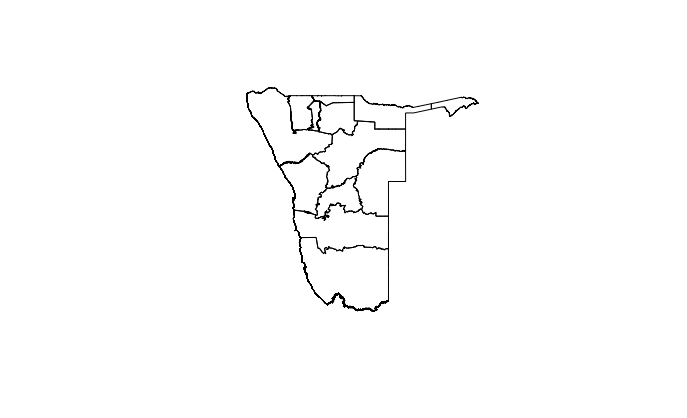
\includegraphics[scale=0.4]{namibia_admin1.png}

\end{frame}

\begin{frame}{Spatial dependence}
One way to visualize discrete spatial structure is to create a \textcolor{blue}{graph} with nodes at the geographic midpoint of each Administrative 1 region, and edges connecting \textit{neighboring} Administrative 1 regions:

\vspace{0.3cm}

\centering 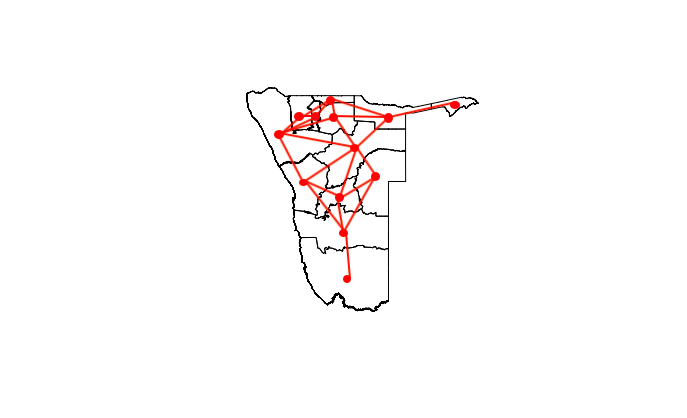
\includegraphics[scale=0.4]{namibia_admin1_2.png}

\end{frame}

\begin{frame}{Spatial dependence}
Let's consider a subset of Namibia Administrative 1 regions in the Northwestern part of the country. We label the regions with numbers below.


\begin{figure}
	\centering 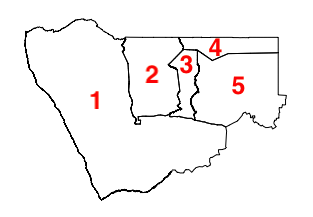
\includegraphics[scale=0.4]{namibia_admin1_subset.png}
\end{figure}

\end{frame}

\begin{frame}{Spatial dependence}

\begin{figure}
	\centering 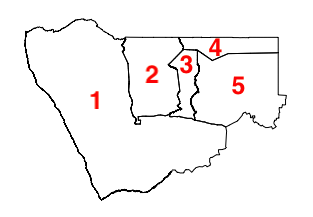
\includegraphics[scale=0.4]{namibia_admin1_subset.png}
\end{figure}

We can record information about the structure of this graph in the following table:

\vspace{0.3cm}

\begin{table}[]
	\begin{tabular}{l|l|l}
		\multicolumn{1}{c|}{Region} & \multicolumn{1}{c|}{Number of Neighbors} & \multicolumn{1}{c}{Neighbors} \\ \hline
		1                           & 3                                        & \{2,3,5\}                     \\
		2                           & 3                                        & \{1,3,4\}                     \\
		3                           & 4                                        & \{1,2,4,5\}                   \\
		4                           & 3                                        & \{2,3,5\}                     \\
		5                           & 3                                        & \{1,3,4\}                    
	\end{tabular}
\end{table}

\end{frame}

\begin{frame}{Spatial dependence}
Without going into too many details, we can transform the information in our table into a matrix, which we can then use to encode spatial dependence into a \textcolor{orange}{spatial random effect}.

\vspace{0.3cm}

What we will eventually end up doing is using this spatial structure along with some parameters (such as a variance parameter) as \textcolor{blue}{prior information} in a Bayesian model. This will allow us to obtain precise predictions of our outcome for all regions in our geographic area, even if we have little to no data in some of those regions.

\vspace{0.3cm}


\includegraphics[scale=0.01]{chilipepper.png} With this particular form of spatial random effect, there is an underlying bias-variance tradeoff going on under the hood here, where we sacrifice some (hopefully negligible) amount of bias for smaller variances (and therefore, more precise predictions).

\end{frame}

\subsection{Bayesian statistics}

\begin{frame}{Bayes' rule, and why it's cool!}
You may recall from BIOST 310 that Bayes' rule is a theorem that relates conditional and mariginal probabilities of events. Suppose we have two events $A$ and $B$. Then Bayes' rule states that
$$
P(A \mid B)  = \frac{P(B \mid A) P(A)}{P(B)}
$$
Bayes' rule is a useful theorem in a variety of statistical applications, but importantly, it is the structural basis of \textcolor{blue}{Bayesian statistics}.

\vspace{0.3cm}

Everything we have done in BIOST 311 falls under the category of \textcolor{orange}{Frequentist statistics}.

\vspace{0.3cm}

\textbf{Fun fact:} Back in the day, statisticians used to get into huge fights over which crowd they fell into (Frequentist or Bayesian). Nowadays, most (reasonable) people agree that both approaches to statistics are useful in different settings.

\end{frame}

\begin{frame}{Bayesian vs. Frequentist statistics}
\small The key difference between Bayesian and Frequentist statistics is whether or not the parameters that you are trying to estimate are \textcolor{orange}{fixed} or \textcolor{blue}{random} variables.

\vspace{0.3cm}

In Frequentist linear regression, recall that the parameters we were trying to estimate were regression coefficients $\beta_0, \dots, \beta_p$. Our estimates of these coefficients were estimates of some \textcolor{orange}{fixed}, unknown, true parameters in the population. This is in part what makes confidence interval interpretations somehwat dissatisfying. 

\vspace{0.3cm}

If we were instead to do Bayesian linear regression, the regression coefficients that we estimate are instead treated as \textcolor{blue}{random} variables with their own probability distributions. For example, rather than $\beta_1$ being a fixed unknown slope coefficient, $\beta_1$ instead would have an entire probability distribution. Rather than a confidence interval for $\beta_1$, we instead get a \textcolor{blue}{credible interval} based on the estimated distribution for $\beta_1$, and the interpretation of the credible interval is the probability that our estimate lies within the interval (a satisfying interpretation!).

\end{frame}

\begin{frame}{Bayesian statistics}
How does all of this relate to Bayes' rule? Let's again consider the case of linear regression. Suppose we have an outcome $Y$ and predictor $X$, and we want to estimate the intercept and slope parameters in our regression. We will estimate both of these parameters as a vector $\beta = (\beta_0, \beta_1)$. Using Bayes' rule, we could write
$$
P(\beta \mid X, Y) = \frac{P(Y \mid X, \beta) P(\beta \mid X)}{P(Y \mid X)}
$$
 A few things to note: \pause

\vspace{0.3cm}
\small 

\begin{itemize}
	\item $P(Y \mid X, \beta)$ should look somewhat familiar to you. Remember that in Chapter 1 we always had $E[Y \mid X, \beta]$ on the left hand side of our regression equation. This piece is similar in Bayesian linear regression!
	\item $P(\beta \mid X, Y)$ is going to be the distribution of our regression coefficients that we are trying to estimate
	\item $P(\beta \mid X)$ is going to be some \textit{prior information} about our regression coefficients that we will use to inform our model
	\item $P(Y \mid X)$ will end up being something we can mostly ignore
\end{itemize}

\end{frame}

\begin{frame}{Bayesian statistics}
In words, we can write Bayes' rule as
$$
\text{Posterior} = \frac{\text{Likelihood} \times \text{Prior}}{\text{Normalizing constant}}
$$
\begin{itemize}
	\item The posterior distribution of our parameters is what we aim to estimate
	\item The likelihood is the contribution of our data to our estimates
	\item The prior contains ``prior" beliefs about our parameters
	\item The normalizing constant makes sure that our posterior distribution is a true probability distribution (a.k.a. that our posterior distribution integrates to 1)
\end{itemize}
\end{frame}

\begin{frame}{Bayesian statistics}
Why would we ever want to do Bayesian statistics?

\vspace{0.3cm}

\begin{itemize}
	\item Bayesian statistics is a natural way of thinking about the world! As humans, we typically have prior beliefs about things, and then we use new information (data) to update those beliefs
	\item \pause Bayesian statistics is especially useful in scenarios where we have good prior information and very little data. Much of Frequentist statistics relies on nice statistical things happening when we have large sample sizes. However, there are certain events in the world that we know will never occur a large number of times (for example, submarine crashes). It may make more sense in these scenarios to do something Bayesian instead
	\item \pause Bayesian statistics can sometimes be computationally more feasible to do than Frequentist statistics. All of the analyses we did in BIOST 311 took very little time to do (probably a few seconds). Many statistical models take \textit{much} longer (days, weeks, \dots) than this to run. This is often true in spatial statistics settings!
\end{itemize}
\end{frame}

\begin{frame}{Bayesian statistics}
How does this relate back to spatial statistics? \pause

\vspace{0.3cm}

In spatial statistics settings, we often have some prior information about the spatial structure of our data (or how strong of a spatial structure our data may have) that we can incorporate into our model in a Bayesian framework. \pause

\vspace{0.3cm}

Additionally, as mentioned on the previous slide, Bayesian statistics is often a much more computationally tractable route when spatial models get complex.
\end{frame}

\section{Cool maps and open statistical questions}

\begin{frame}{Cool maps!}
On the next few slides, there are examples of cool maps we can make of the predictions we obtain using Bayesian spatial models for Under-5 Mortality estimation for the UN and HIV prevalence estimation for a project related to spatial statistics methodology development.
\end{frame}

\begin{frame}{Under-5 Mortality Estimation for the UN}
\centering 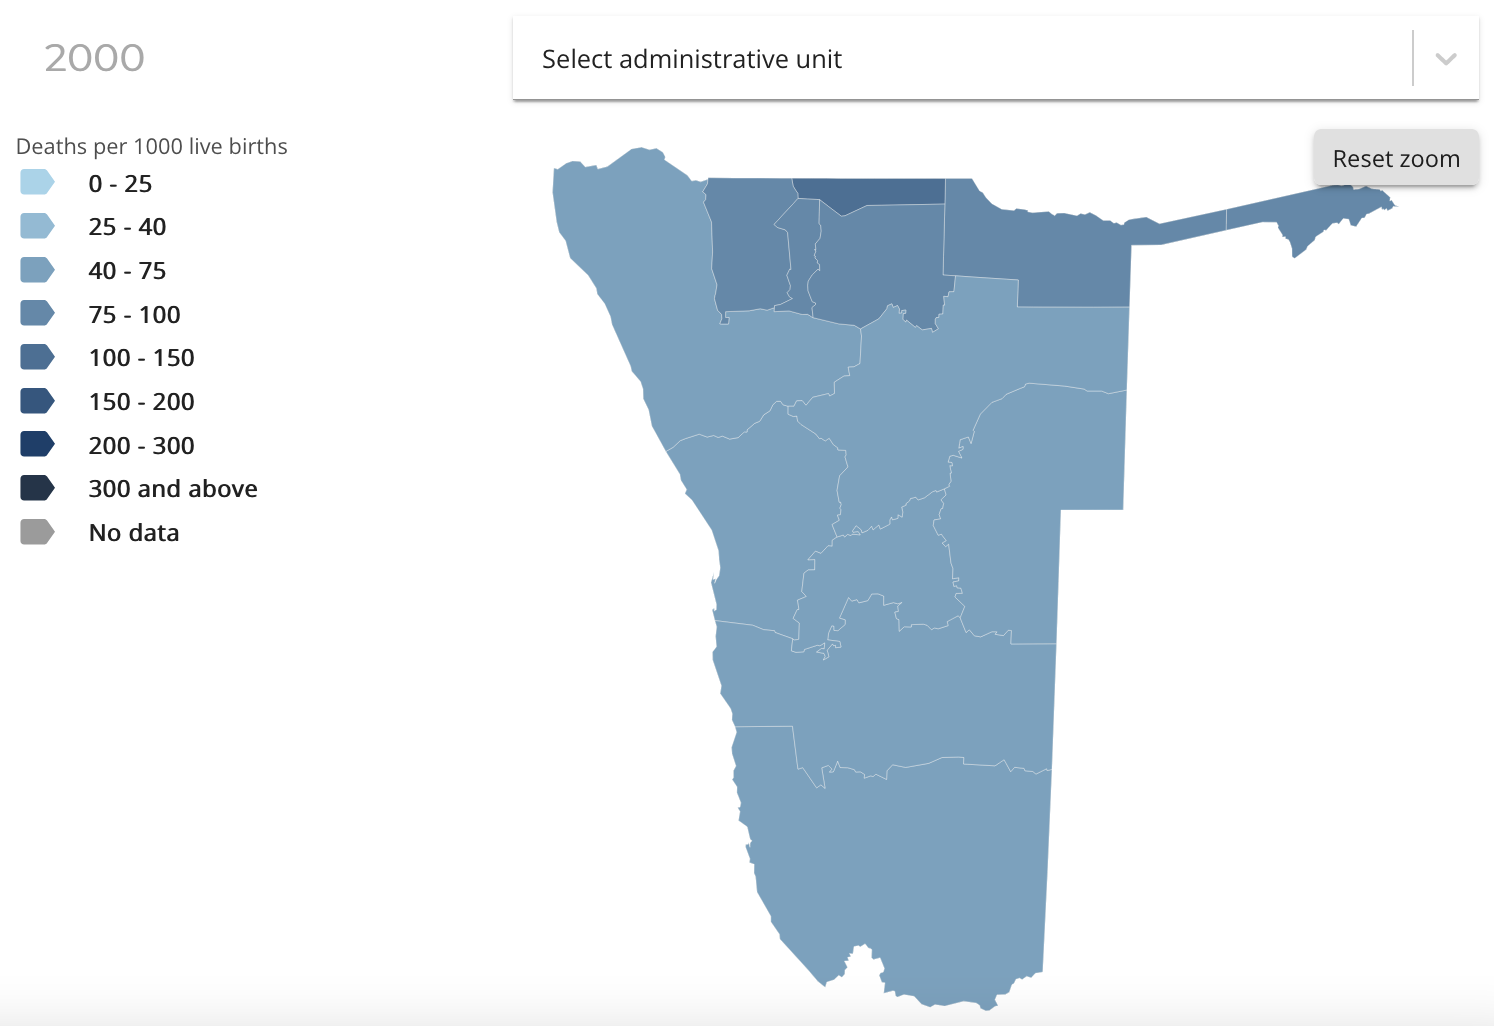
\includegraphics[scale=0.4]{namibia_igme.png}
\end{frame}

\begin{frame}{HIV Prevalence estimation in South Africa}
\centering 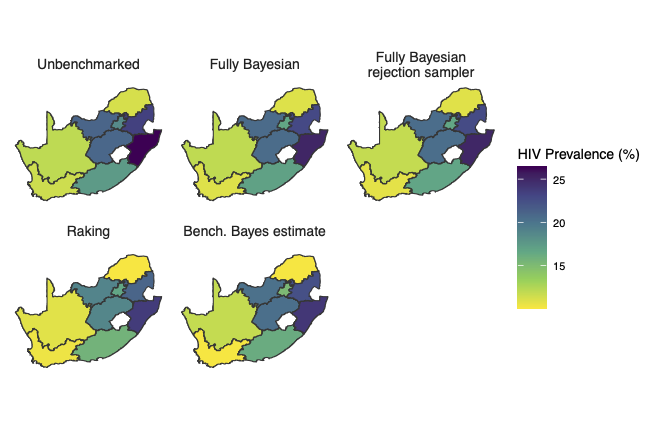
\includegraphics[scale=0.4]{map_compare_medians.png}
\end{frame}

\begin{frame}[c]{HIV Prevalence estimation in South Africa}
\centering 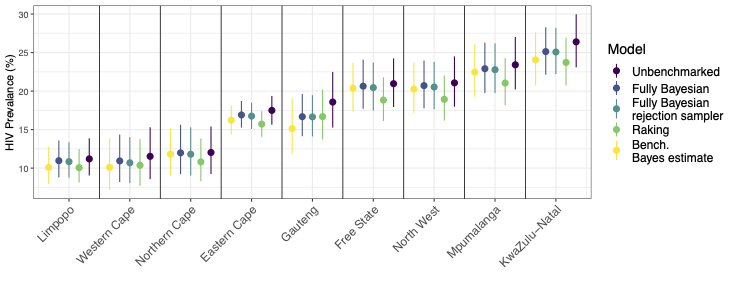
\includegraphics[scale=0.4]{ranking_plot.png}
\end{frame}

\begin{frame}{Open statistical questions}
Examples of spatial statistics and under-5 mortality research questions that have yet to be answered in a satisfying way:

\vspace{0.3cm}

\begin{itemize}
	\item How do we combine vital registration, full birth history, and summary birth history data to produce predictions of under-5 mortality?
	\item How do we encode spatial dependence into a statistical model for countries that contain islands (if at all)?
	\item How do we incorporate fertility and migration information into models for under-5 mortality?
	\item How do we adequately account for the design of DHS (or other) surveys in our statistical models when we have little to no data in certain regions?
	\item How do we improve the computational speed of our models so that statisticians in national statistical offices in low and middle income countries can produce their own estimates?
	\item Many more!
\end{itemize}

\end{frame}


\end{document}